\documentclass[letterpaper]{article}
\usepackage{aaai}
\usepackage{times}
\usepackage{helvet}
\usepackage{courier}
\usepackage{graphicx}
\usepackage{hyperref}
\hypersetup{
    colorlinks=true,
    linkcolor=blue,
    filecolor=magenta,
    urlcolor=cyan,
}
\frenchspacing
\setlength{\pdfpagewidth}{8.5in}
\setlength{\pdfpageheight}{11in}
\setcounter{secnumdepth}{0}
%\documentclass[twoside]{uva-inf-bachelor-thesis}
%\usepackage[dutch]{babel}

% Filling your thesis with only lorem ipsum is not advised.
\usepackage{amsmath}
\makeatletter
\newcommand{\tpmod}[1]{{\@displayfalse\pmod{#1}}}
\makeatother

\usepackage[
backend=biber,
style=alphabetic,
sorting=ynt
]{biblatex}

\addbibresource{bibliography.bib}

\begin{document}

% Title Page
\title{Sudoku SAT solver}
\author{Theofilos Papapanagiotou, Hung Nguyen}
%\supervisors{drs. W. Beek, prof. dr. Frank van Harmelen}
%\signedby{Signees}

\maketitle
% \begin{abstract}
% \lipsum[2]
% \end{abstract}

% \tableofcontents

\href{https://www.youtube.com/watch?v=tk7kIJBqUiQ}{Video presentation} of the report is available.

\section{Hypothesis}
Enriching the encoding of a Sudoku as a SAT-problem, will improve the performance of the SAT-solver by decreasing the conflicts, propagation's and decisions.
The intuition here is that enriching the encoding by adding more constraints, will decrease the search space. This will in turn improve performance by decreasing the amount of conflicts, propagation's and decisions.
This experiment aims to find out how different representations of the same problem might perform differently performance-wise. It is interesting to identify which type of encoding technique has the most influence on the performance. We will not only be looking at different ways to encode the Sudoku rules themselves, but also in ways to exploit the assigned variables to do some Sudoku-specific optimizations.

\section{Experimental setup}
\subsection{Tools}
To get something meaningful statistics from the experiment, a SAT-solver was needed that keeps track of the statistics. For this, the existing SAT-solver MiniSAT\cite{sorensson2005minisat} was chosen. This is a minimalistic, high-performance and easy-to-use SAT solver that fulfilled the requirements.\\
To accurately measure the performance of different Sudoku-to-SAT encodings, these had to be created from scratch to ensure it's correct implementation.
\subsection{Implementation}
The rules of Sudoku are as follows:
\begin{enumerate}
    \item Each cell must contain a digit from 1 to n
    \item Each cell can only contain a single digit
    \item Each row must contain all digits from 1 to n
    \item Each row cannot contain the same digit twice or more
    \item Each column must contain all digits from 1 to n
    \item Each column cannot contain the same digit twice or more
    \item Each region must contain all digits from 1 to n
    \item Each region cannot contain the same digit twice or more
\end{enumerate}
These same rules can used to represent a Sudoku problem as a SAT problem, by translating them using propositional logic. We use a variable $v_{rc}$ to represent a value $v$ at row index $r$ and column index $c$. \\
This encoding is similar to the encoding introduced by \cite{kwon2006optimized}. However, their way of encoding the block constraints didn't work correctly and was very unclear. Therefore, we used our own.\\

$cell_d$: each cell must contain a digit from 1 to n
$$
\bigwedge_{r=1}^{n}\bigwedge_{c=1}^{n}\bigvee_{v = 1}^{n} v_{rc}
$$
$cell_u$: each cell can only contain a single digit
$$
\bigwedge_{r=1}^{n}\bigwedge_{c=1}^{n}\bigwedge_{v_i = 1}^{n-1}\bigvee_{v_j = v_i+1}^{n} \neg v_{i_{rc}} \vee \neg v_{j_{rc}}
$$
$row_d$: each row must contain all digits from 1 to n
$$
\bigwedge_{r=1}^{n}\bigwedge_{v=1}^{n}\bigvee_{c = 1}^{n} v_{rc}
$$
$row_u$: each row cannot contain the same digit twice or more
$$
\bigwedge_{r=1}^{n}\bigwedge_{v=1}^{n}\bigwedge_{c_i=1}^{n-1}\bigvee_{c_j = c_i+1}^{n} \neg v_{rc_i} \vee \neg v_{rc_j}
$$
$col_d$: each column must contain all digits from 1 to n
$$
\bigwedge_{c=1}^{n}\bigwedge_{v=1}^{n}\bigvee_{r = 1}^{n} v_{rc}
$$
$col_u$: each column cannot contain the same digit twice or more
$$
\bigwedge_{c=1}^{n}\bigwedge_{v=1}^{n}\bigwedge_{r_i=1}^{n-1}\bigvee_{r_j = r_i+1}^{n} \neg v_{r_ic} \vee \neg v_{r_jc}
$$
$block_d$: each region must contain all digits from 1 to n
$$
\bigwedge_{v=1}^{n}\bigwedge_{g=1}^{n}\bigvee_{r=\sqrt{n} \cdot \frac{g}{\sqrt{n}}}^{\sqrt{n} \cdot (\frac{g}{\sqrt{n}} + 1)}\bigvee_{c=\sqrt{n} \cdot (g \tpmod{\sqrt{n}}) }^{\sqrt{n} \cdot (g\tpmod{\sqrt{n}} + 1)} v_{rc}
$$
(note: here we assume integer division)\\
$block_u$: each region cannot contain the same digit twice or more
$$
\bigwedge_{v=1}^{n}\bigwedge_{g=1}^{n}\bigwedge_{r_i=\sqrt{n} \cdot \frac{g}{\sqrt{n}}}^{\sqrt{n} \cdot (\frac{g}{\sqrt{n}} + 1)}\bigwedge_{c_i=\sqrt{n} \cdot (g \tpmod{\sqrt{n}}) }^{\sqrt{n} \cdot (g\tpmod{\sqrt{n}} + 1)} \bigvee_{r_j=r_i+1}^{\sqrt{n} \cdot (\frac{g}{\sqrt{n}} + 1)}\bigvee_{c_j=c_i + 1}^{\sqrt{n} \cdot (g\tpmod{\sqrt{n}} + 1)} \neg v_{r_ic_i} \vee \neg v_{r_jc_j}
$$
(note: here we assume integer division)\\

Using these constraints, the rules of Sudoku can be representing in the following three encodings:
$minimal = cell_d \wedge row_u \wedge block_u \wedge assigned$\\
$efficient = cell_d \wedge cell_u \wedge row_u \wedge col_u \wedge block_u \wedge assigned$\\
$extended = cell_d \wedge cell_u \wedge row_d \wedge row_u \wedge col_d \wedge col_u \wedge block_d \wedge block_u \wedge assigned$\\
\subsection*{Optimization's}
Taking advantage of the fact that this is a Sudoku-problem, a few optimization's can be performed for every known cell $v_{rc}$ in the Sudoku. These are all implied clauses, which can be removed beforehand. We refer to the encodings with the implied clauses removed, as the optimized encodings. \\

All other cells on the same column are not number $v$:
$$
\bigwedge_{v_i=1}^{n} \neg v_{i_{rc}} \textbf{ if } v_i \neq v
$$

All other cells on the same column are not number $v$:
$$
\bigwedge_{r_i=1}^{n} \neg v_{r_{i}c} \textbf{ if } r_i \neq r
$$

All other cells on the same row are not number $v$:
$$
\bigwedge_{c_i=1}^{n} \neg v_{rc_i} \textbf{ if } c_i \neq c
$$

All other cells in the same region are not number $v$:
$$
\bigwedge_{r_i = \sqrt{n} * \frac{r}{\sqrt{n}}}^{\sqrt{n} * (\frac{r}{\sqrt{n}} + 1)}
\bigwedge_{c_i = \sqrt{n} * \frac{c}{\sqrt{n}}}^{\sqrt{n} * (\frac{c}{\sqrt{n}} + 1)}
\neg v_{r_{i}c_{i}} \textbf{ if } r_i \neq r \textbf{ and } c_i \neq c
$$
(note: assuming integer division)\\

\section{Experimental results}

Given the output results collected by the execution of the SAT solver using minisat, we are reporting the performance of the 6 different encodings. The selected metrics which we are using to report the performance, are the number of conflicts, restarts, decisions, propagations and conflict literals.

\begin{figure}
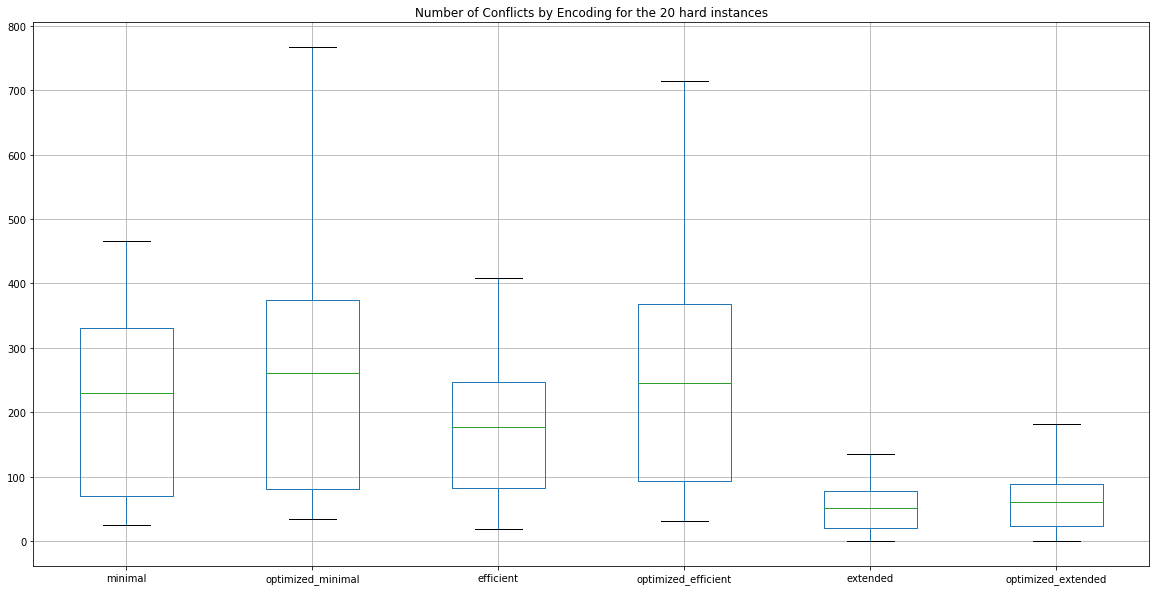
\includegraphics[scale=0.2]{conflicts.png}
\caption{Graph of the conflicts}
\end{figure}

\begin{figure}
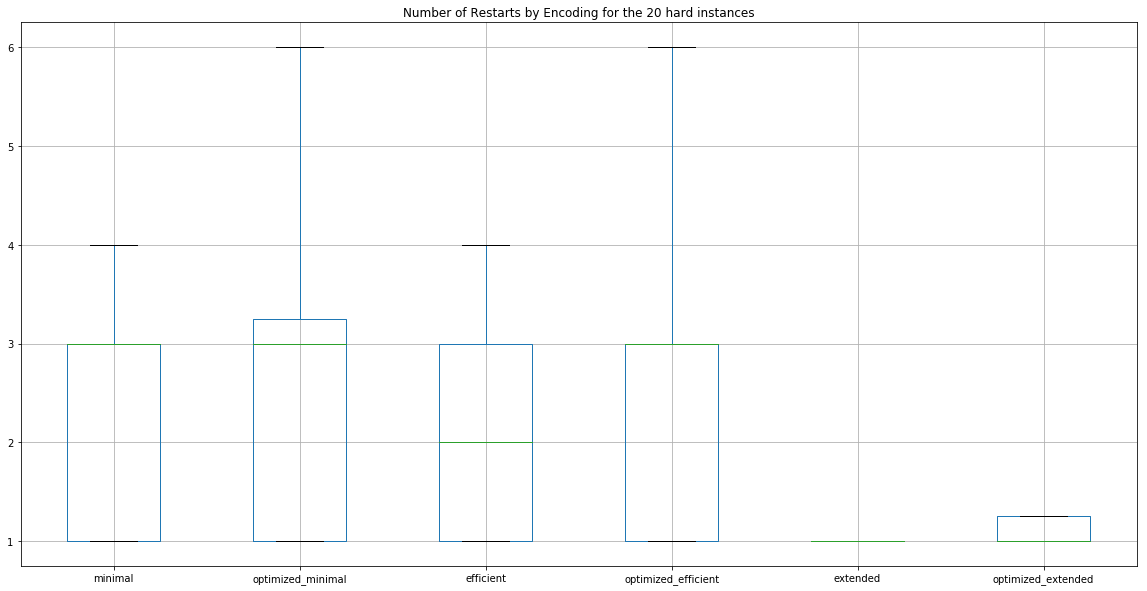
\includegraphics[scale=0.2]{restarts.png}
\caption{Graph of the restarts}
\end{figure}

\begin{figure}
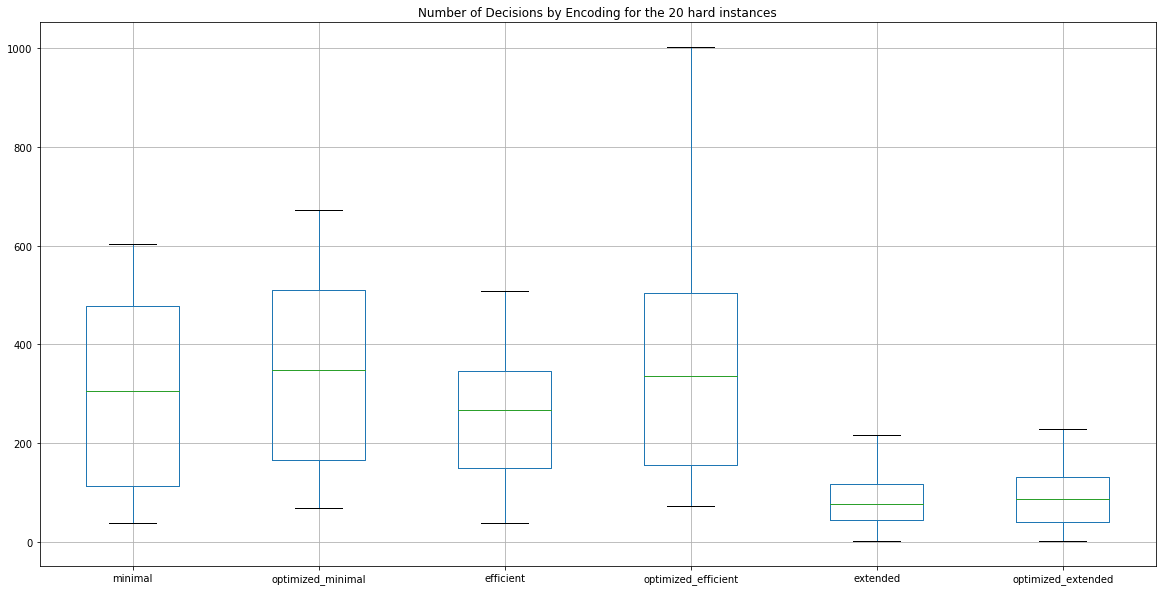
\includegraphics[scale=0.2]{decisions.png}
\caption{Graph of the decisions}
\end{figure}

\begin{figure}
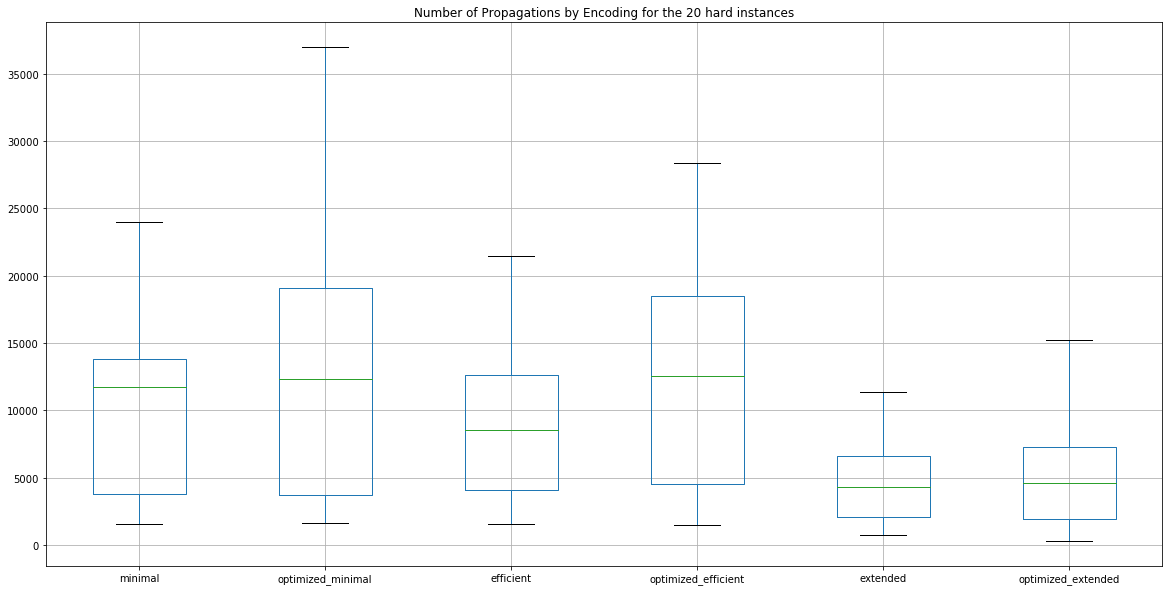
\includegraphics[scale=0.2]{propagations.png}
\caption{Graph of the propagations}
\end{figure}

\begin{figure}
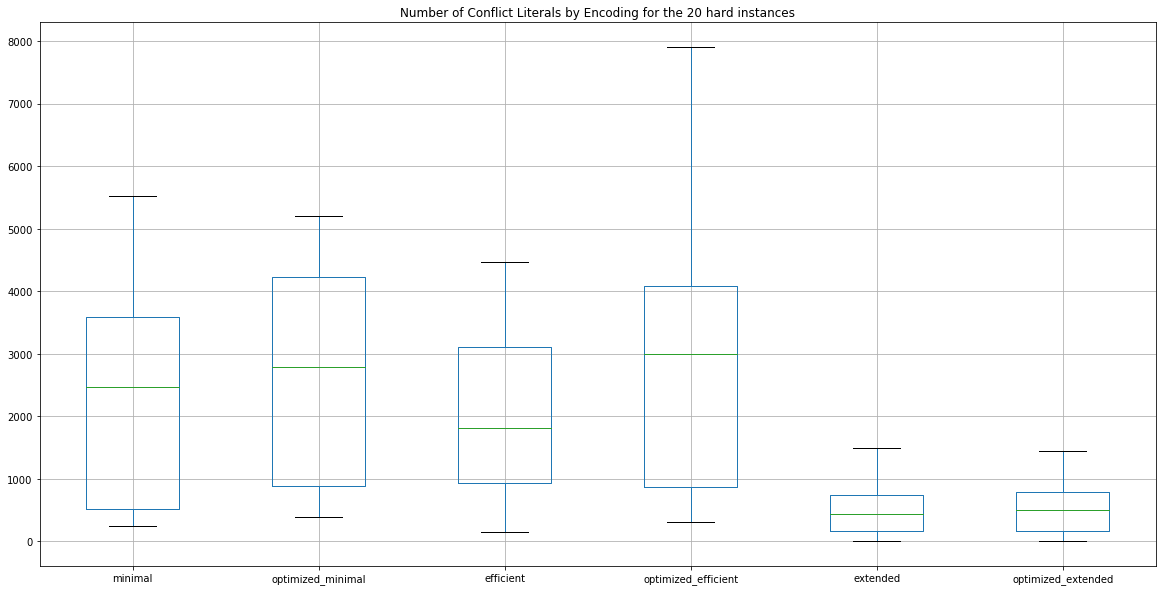
\includegraphics[scale=0.2]{conflict_literals.png}
\caption{Graph of the conflict literals}
\end{figure}

The size of the selected dataset is small, only 20 hard instances have been used. In order to validate the hypothesis with more certainty, we could have used a larger dataset with 17 givens, still choosing from hard instances \cite{selman1992new} \cite{selman1996generating}.

The selection of the performance metrics was based in the available report of the chosen tool \cite{sorensson2005minisat}. A more recent SAT Solver \cite{soos2016cryptominisat} reports more metrics, based on the same basic indicators we have used in this project, but examining them during the execution and in relation to each other.

The evaluation of a larger dataset in combination with the extended indicators would provide more concrete results for this measurement.


\section{Interpretation}

The experimental results confirm our hypothesis. The 5 chosen metrics show improved performance, as the numbers of the metrics are lower in the more efficient encodings.
Especially the group of the two \textbf{extended} encodings which contains the more complete set of clauses, outperforms the groups of \textbf{minimal} and \textbf{efficient} encodings. The \textbf{minimal} and \textbf{efficient} encodings compared to each other, do not have large differences in the observed metrics.
The introduction of the optimization step to eliminate the literals and the clauses, did not improve much the performance of the SAT solver compared to the execution without these steps.

\section{Conclusion summary}

It was expected that the introduction of more constraints will decrease the search space and improve the performance metrics we have chosen.

The dataset and tools used can be improved to increase the certainty of the hypothesis. Additional heuristics can be used to create a wide range of different improvement steps.

\printbibliography

\end{document}
